\paragraph{}{
	Le banc de registres constitue la mémoire du processeur.
	Il est composé 16 registres d'un octet. Un tel circuit
	est composé de bascules D en cascade. Il y en a une pour
	chaque registre.
	L'écriture d'un registre est possible uniquement lorsque
	\textit{regWrite} est à vrai.
}

\begin{figure}
	\centering
	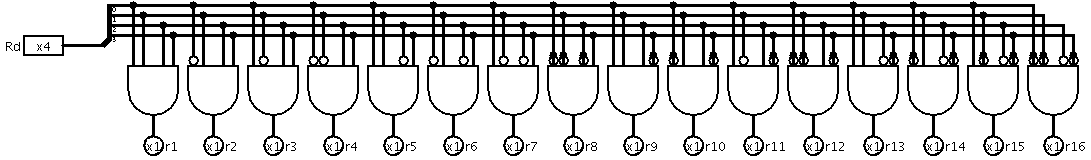
\includegraphics[scale=0.3,angle=90,origin=c]{circuits/banc_reg.png}
	\label{banc_reg_circ}
	\caption{Sch\'{e}ma \'{e}lectronique pour le banc de registres}
\end{figure}

\begin{figure}
	\centering
	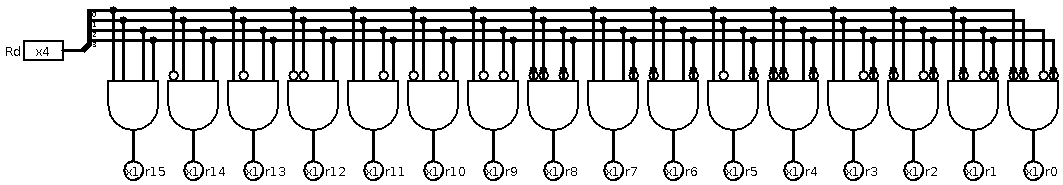
\includegraphics[scale=0.3,origin=c]{circuits/banc_reg_selec.png}
	\caption{
		\label{banc_reg_selec_circ}
		Sch\'{e}ma \'{e}lectronique pour le sélecteur du banc de registres
	}
\end{figure}